\documentclass[12pt,a4paper]{article}
\usepackage{algorithm, algpseudocode, amsmath, amssymb, amsthm, bm, csquotes, emf, empheq, geometry, graphicx, hyperref, listings, mhchem, multirow, siunitx, slashbox, subcaption, upgreek}
\usepackage[italicdiff]{physics}
\usepackage[section]{placeins}
\usepackage[justification=centering]{caption}
\usepackage[column=O]{cellspace}
\usepackage[extrafootnotefeatures]{xepersian}
\hypersetup{colorlinks=true, urlcolor=cyan}

\title{آزمایش کنارتاریکی خورشید}
\author{آرتین خانعلی، سپهر سلمانی یگانه، صالح شاملو احمدی\\\\
	آزمایشگاه نجوم، ترم تابستان ۱۴۰۲\\دانشکده فیزیک دانشگاه صنعتی شریف}
\date{۳۱ تیر ۱۴۰۲}

\settextfont{Yas}
\ExplSyntaxOn
\cs_set_eq:NN
\etex_iffontchar:D
\tex_iffontchar:D
\cs_undefine:N \c_one
\int_const:Nn \c_one { 1 } 
\ExplSyntaxOff
\setdigitfont{Yas}
\linespread{1.2}

\makeatletter
\g@addto@macro\bfseries{\boldmath}
\makeatother

\setlength\cellspacetoplimit{5pt}
\setlength\cellspacebottomlimit{3pt}
\newcommand{\multlinecell}[1]{\begin{tabular}[c]{@{}c@{}}#1\end{tabular}}

\newcommand{\qfrac}[2]{\left(\frac{#1}{#2}\right)}
\newcommand{\fsqrt}[2]{\sqrt{\frac{#1}{#2}}}
\newcommand{\ddfrac}[2]{{\displaystyle\frac{\displaystyle #1}{\displaystyle #2}}}
\newcommand{\pdvc}[3]{\qfrac{\partial #1}{\partial #2}_{#3}}
\newcommand{\dbar}{{d\mkern-7mu\mathchar'26\mkern-2mu}}
\newcommand*{\defeq}{\mathrel{\vcenter{\baselineskip0.5ex \lineskiplimit0pt
			\hbox{\scriptsize.}\hbox{\scriptsize.}}}
	=}

\newtheorem{theorem}{قضیه}
\newtheorem{lemma}{لم}
\renewcommand\qedsymbol{$\blacksquare$}

\begin{document}
	\maketitle
	\twocolumnfootnotes
	\section{مقدمه}
	در این آزمایش، با پردازش عکس‌های تهیه شده از خورشید، اثر کنارتاریکی\footnote{\lr{limb darkening}} را بررسی می‌کنیم.
	عکس‌های خورشید توسط استاد و دستیاران آموزشی درس تهیه شده‌اند و در اینجا به جزئیات آن نمی‌پردازیم.
	\section{ابزار استفاده‌شده}
	\begin{itemize}
		\item تلسکوپ ۶ اینچی نیوتونی
		\item دوربین \lr{Canon EOS 1200D}
		\item فیلتر خورشیدی
	\end{itemize}
	\section{نظریه}
	\begin{figure}
		\centering
		\includegraphics[width=\linewidth]{../fig/Limb_darkening_layers.pdf}
		\caption{توضیح اثر کنارتاریکی. نور مربوط به طول ثابتی از سطح از نظر ناظری در بی‌نهایت، از لایه کم‌دماتر می‌آید.}
		\label{fig:limbdark}
	\end{figure}
	کنارتاریکی به این دلیل رخ می‌دهد که در گوشه‌ی خورشید، نور توسط مقدار پلاسمای کمتر در دمای سردتری ساطع می‌شود.
	می‌توانید به‌صورت تصویری این موضوع را در شکل \ref{fig:limbdark} مشاهده کنید.
	
	طبق تقریب ادینگتون، با در نظر گرفتن اثر کنارتاریکی، پروفایل روشنایی خورشید از رابطه
	\begin{equation}
		\frac{I(\mu)}{I(0)} = \frac{2 + 3\mu}{5}
	\end{equation}
	بدست می‌آید که $\mu = \cos\theta$ و $\theta$ زاویه خط واصل نقطه مورد نظر روی قرص خورشید و مرکز خورشید با
	خط واصل مرکز قرص خورشید و مرکز خورشید است. این رابطه با فرض اینکه شعاع خورشید به‌نسبت فاصله زمین از خورشید
	قابل صرف‌نظر است بدست آمده (یعنی به اندازه‌ای نیست که روی زاویه پرتوها تأثیر قابل‌توجهی بگذارد). همچنین
	این تقریب بر پایه مدل ادینگتون از خورشید است که فرض می‌کند خورشید چگالی ثابت دارد.
	\section{پیش‌پردازش}
	در این آزمایش عکس صفحه تخت\footnote{\lr{flat frame}} نداشتیم و فقط عکس‌های جریان تاریک\footnote{\lr{dark current}}
	در دسترس داشتیم.
	
	قبل از هر چیز، تصاویر خام دوربین با فرمت \lr{\tt{CR2}} را به فرمت \lr{\tt{fits}} تبدیل کردیم. چون خروجی دوربین
	به‌صورت \lr{rgb} نیست اما ما این فرمت را تحلیل و پردازش می‌کنیم، در این مرحله به الگوریتمی برای
	غیرموزائیکی‌کردن\footnote{\lr{demosaicing}} نیاز داریم. خوشبختانه الگوریتم‌های پیشرفته فراوانی برای این منظور
	طراحی شده اند. در حال حاضر \lr{AMaZE} پراستفاده‌ترین الگوریتم غیرموزائیکی‌کردن است، اما ما از الگوریتم \lr{RCD}
	استفاده می‌کنیم که برای لبه‌های نرم در تصویر بهتر عمل می‌کند و پیش‌فرض بعضی نرم‌افزارهای رصدی نیز هست. بعد از
	غیرموزائیکی کردن، کافی است با تبدیل ساختار پیکسل‌ها به استاندارد \lr{fits} و همچنین استخراج
	فراداده‌های\footnote{\lr{metadata}} دوربین و قرار دادن آن با بقیه اطلاعات مربوطه در \lr{header} فایل، داده‌ها
	را در فرمت \lr{\tt{fits}} ذخیره کنیم.
	
	در مرحله اول پیش‌پردازش، از عکس‌های جریان تاریک میانه گرفتیم که عکس \lr{master} جریان تاریک را درست کنیم.
	سپس مقادیر این عکس را از عکس اصلی کم کردیم تا نویز بایاس و جریان تاریک از عکس اصلی حذف شوند.
	
	مرحله بعدی، پیداکردن پیکسل‌های «بد» است؛ پیکسل‌های داغ با کم کردن جریان تاریک اصلاح می‌شوند، اما پیکسل‌های بد کاملاً
	سوخته‌اند و واکنش درست به نور نشان نمی‌دهند. برای پیدا کردن این پیکسل‌ها، از جریان تاریک مربوط به نوردهی دیگری
	کمک می‌گیریم. در این رصد برای عکس‌بردار از خورشید از نوردهی $1/30$ ثانیه استفاده کردیم و جریان تاریک اصلی هم
	مربوط به همین نوردهی بوده، اما علاوه بر آن جریان تاریک مربوط به نوردهی $0.01$ ثانیه را هم گرفته‌ایم. ابتدا پیکسل‌های
	داغ را پیدا می‌کنیم. با یک نگاه اجمالی به هیستوگرام فراوانی شدت پیکسل‌ها، برای هر کانال یک حد برای «داغ» بودن انتخاب
	می‌کنیم. این حد برای کانال قرمز $8$، برای کانال سبز $1$، و برای کانال آبی $4$ واحد است. با رسم شدت پیکسل‌های داغ روی
	روی نوردهی $1/30$ ثانیه برحسب شدت روی نوردهی $0.01$ ثانیه، نمودار \ref{fig:hotpix} بدست می‌آید. می‌بینیم که بیشتر
	نقاط تقریباً روی یک خط می‌افتند، به جز چند نقطه پرت. این نقطه‌های پرت، همان پیکسل‌های سوخته هستند. برای پیدا کردن
	آن‌ها، ابتدا سعی می‌کنیم خطی که از بیشتر نقطه‌ها عبور می‌کند را پیدا کنیم. این کار آنقدری که در نگاه اول به نظر
	می‌رسد ساده نیست، چراکه نقطه‌های پرت متقارن نیستند و شیب خط را به‌شدت تحت‌تأثیر قرار می‌دهند. از نظر تئوری،
	در نوردهی‌های بالا این شیب باید برابر نسبت نوردهی‌ها باشد، اما در اینجا چون به‌نسبت نوردهی کم است، نویز
	خوانش\footnote{\lr{read noise}} و بایاس تأثیر زیادی دارند. در آخر با کمی سعی و خطا می‌توان شیب اصلی را پیدا کرد
	که در اینجا حدود $1.3$ است. حال که خط را پیدا کردیم، نقاطی که بیش از $30$ درصد از این خط فاصله دارند را به عنوان
	پیکسل بد در نظر می‌گیریم. البته پیکسل‌هایی که شدت کمی دارند (در اینجا زیر $65$ واحد) را در نظر نمی‌گیریم چون
	به اندازه‌ی کافی برای یک پیکسل سوخته شدت بالایی ندارند. اینکه چه حدی برای این \lr{cut-off} مناسب است، زیاد دقیق
	نیست اما در کل دسته پیکسل‌های کم‌شدت به هم چسبیده را در نظر نمی‌گیریم. بعد از پیدا کردن پیکسل‌های سوخته، آن‌ها را با
	یک ماسک از تحلیل‌های بعدی خارج می‌کنیم.
	
	\begin{figure}
		\centering
		\begin{subfigure}{0.49\linewidth}
			\centering
			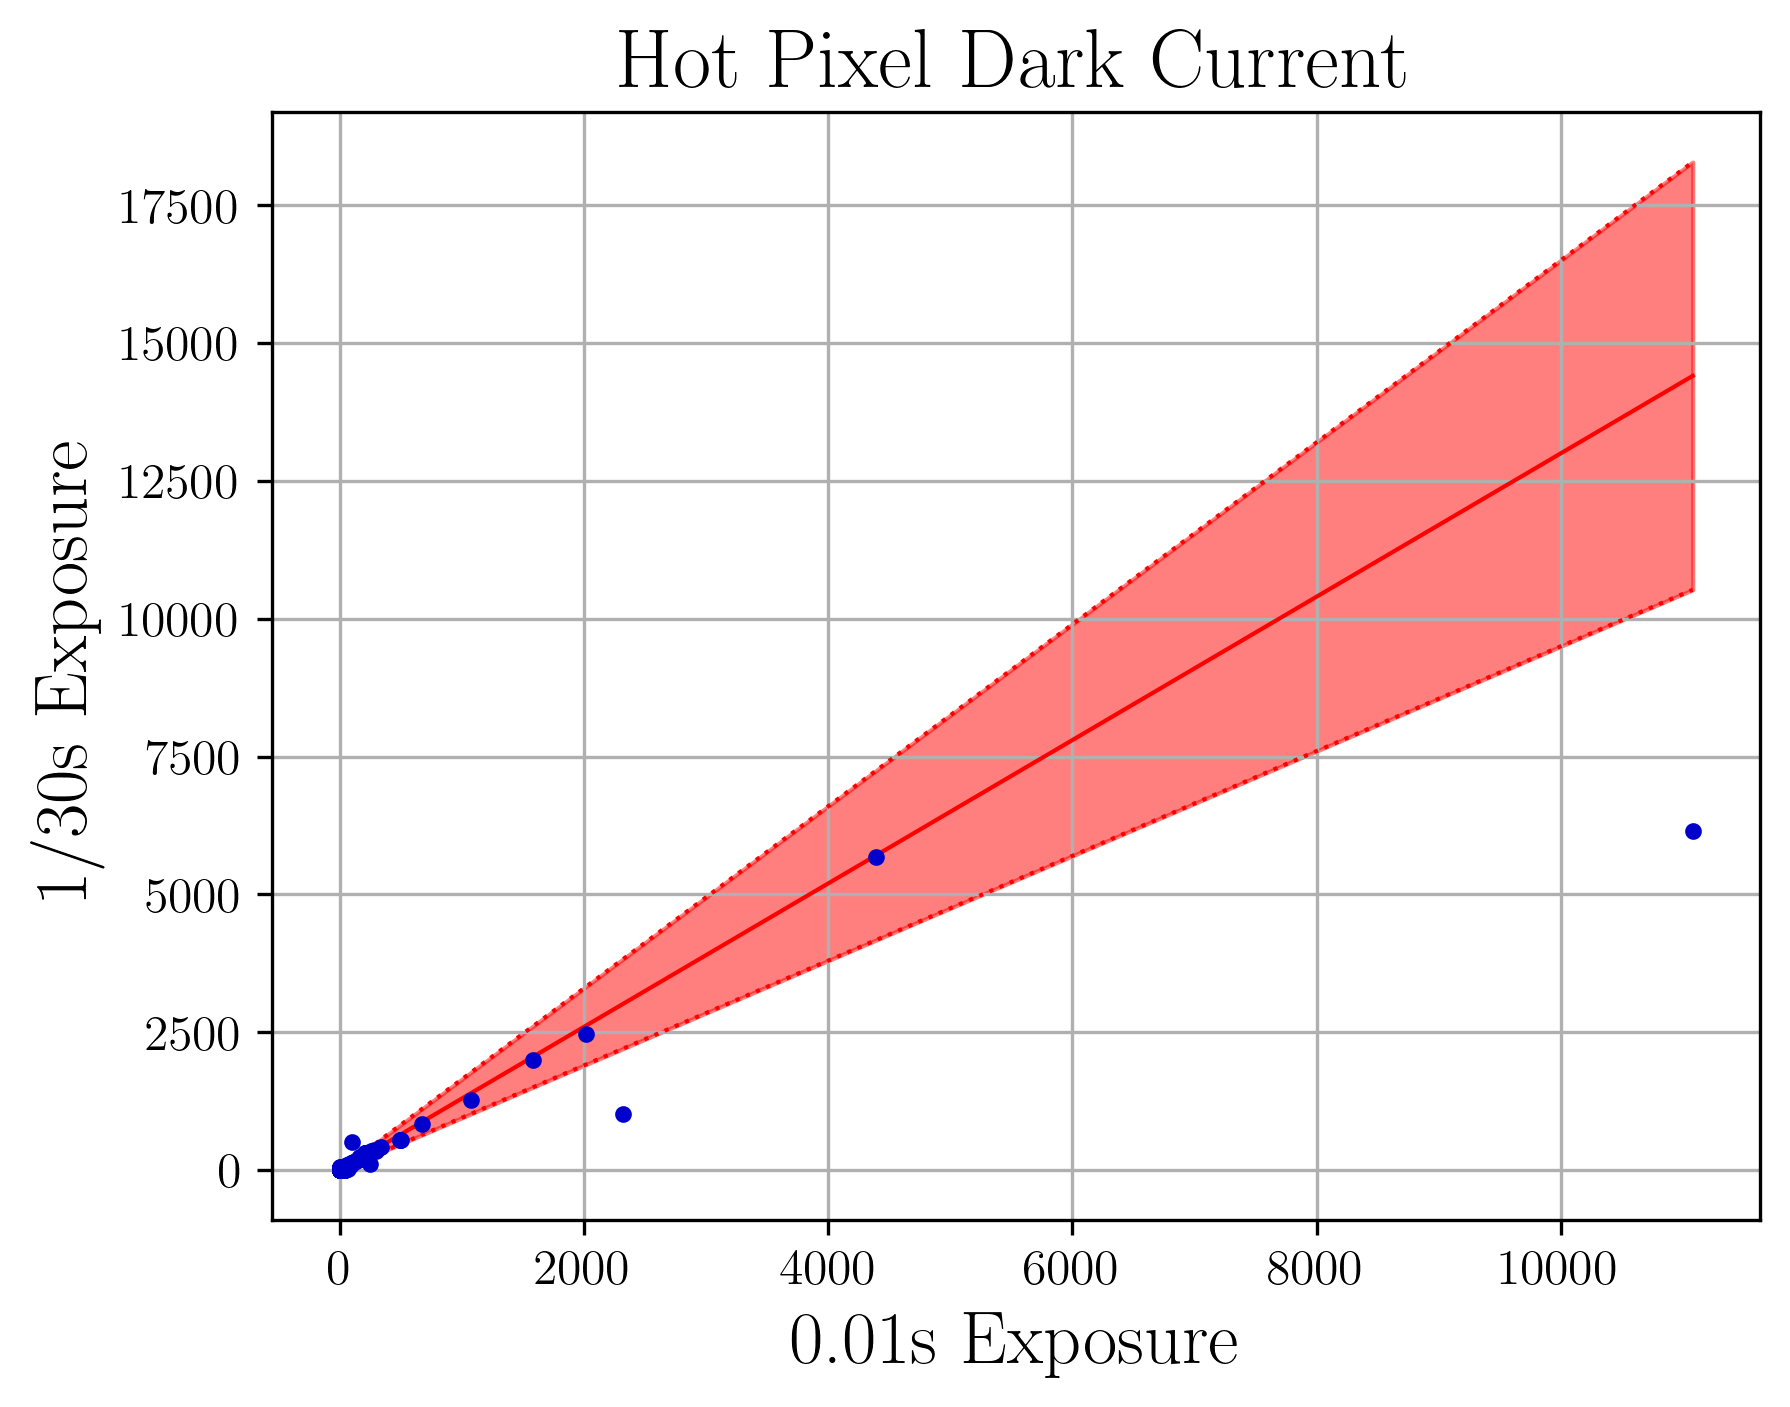
\includegraphics[width=\linewidth]{../fig/hotpix}
		\end{subfigure}
		\begin{subfigure}{0.49\linewidth}
			\centering
			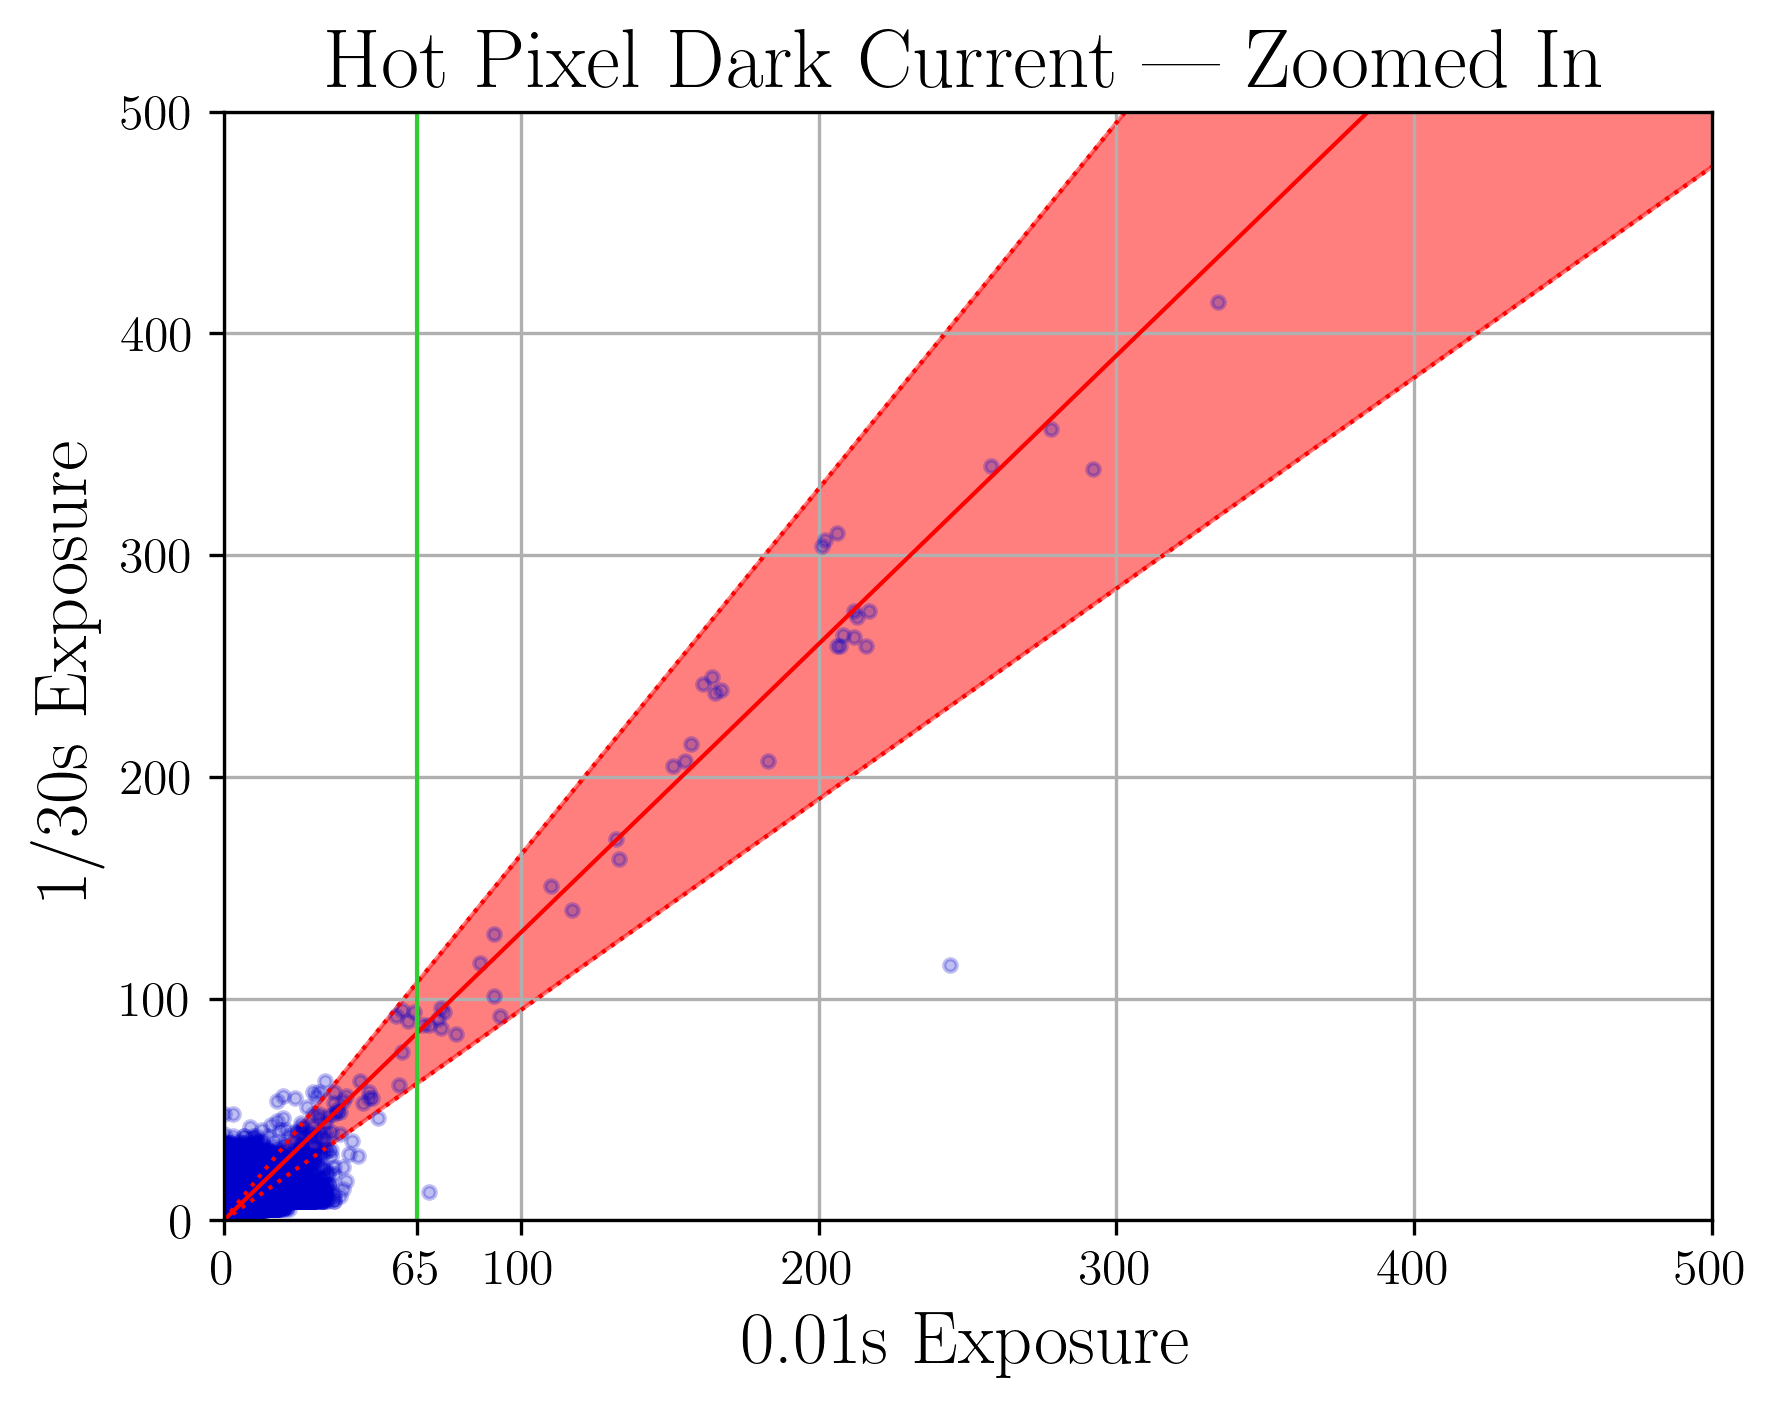
\includegraphics[width=\linewidth]{../fig/hotpix-zoom}
		\end{subfigure}
		\caption{پراکندگی پیکسل‌های داغ روی نمودار دو شدت. محدوده رنگی، محدوده مجاز است. نقاط پیش از خط سبز
			در نظر گرفته نمی‌شوند.}
		\label{fig:hotpix}
	\end{figure}
	
	در آخر کانال‌های قرمز و سبز و آبی را یکی می‌کنیم (به عبارتی تصویر را «خاکستری» (\lr{grayscale}) می‌کنیم) و مقادیر
	پیکسل‌ها را بهنجار می‌کنیم. خاکستری کردن تصویر و بهنجارش روشنایی‌ها، تحلیل را ساده‌تر می‌کنند. البته که اگر از سه
	کانال رنگی مختلف، نیاز داشته باشیم داده‌های مختلف بگیریم، نباید کانال‌ها را ترکیب کنیم، اما در این آزمایش نیازی
	به تمام اطلاعات نداریم و فقط روشنایی کلی برای‌مان مهم است. تصاویر را در مرحله اول در فضای رنگی \lr{sRGB} ذخیره
	کردیم، بنابراین از رابطه تبدیل \lr{sRGB} به \lr{grayscale} استفاده می‌کنیم.
	\begin{equation}
		\text{\lr{grayscale intensity}} = 0.2126r + 0.7152g + 0.0722b
	\end{equation}
	این رابطه صرفاً روشنایی نسبی مربوط به چشم انسان که از هر رنگ دیده می‌شود را در نظر می‌گیرد. برای بهنجارش روشنایی
	هم کافیست روشنایی هر پیکسل را بر بیشینه روشنایی پیکسل‌ها تقسیم کنیم.

	\section{پیدا کردن شعاع و مرکز}
	اینکه «لبه» خورشید دقیقاً کجا قرار دارد، پاسخ دقیقی ندارد. حتی با استفاده از پروفایل روشنایی، ممکن است جایی را
	انتخاب کنیم که به چشم انسان از لبه دور باشد. بنابراین مجبوریم این بخش را تقریبی انجام دهیم. ما چشمی در نظر گرفتیم
	پیکسل‌هایی که بیش از $15$ درصد روشنایی دارند، داخل خورشید قرار دارند. با تقسیم فاصله بیشینه و کمینه‌ی $x$ و $y$ این
	نقاط بر دو، شعاع خورشید بدست می‌آید. ما با این روش شعاع خورشید را $799$ پیکسل بدست آوردیم.
	\begin{figure}
		\centering
		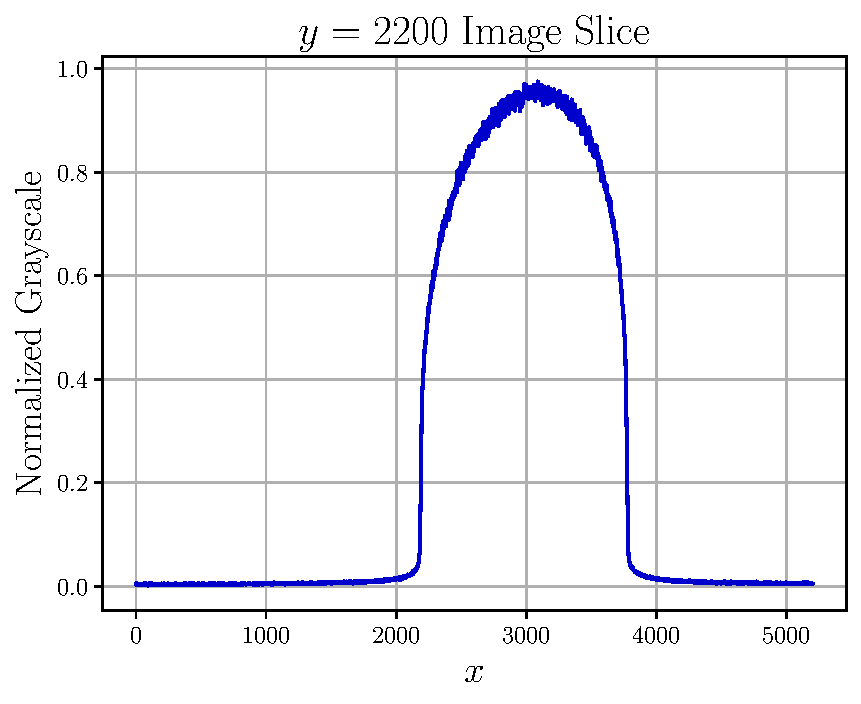
\includegraphics[width=0.8\linewidth]{../fig/slice}
		\caption{پروفایل روشنایی استفاده‌شده برای پیدا کردن شدت پیکسل‌های خورشید.}
	\end{figure}
	برای پیدا کردن مرکز خورشید روش‌های متعددی وجود دارد. روش‌های هندسی مثل پیدا کردن تقاطع عمود منصف وتر‌ها یا تقاطع
	عمود‌های دو مماس خورشید به‌نسبت دقیق هستند. وسط بیشینه و کمینه‌ی $x$ و $y$ مرکز خورشید را نشان می‌دهد که
	روش هندسی دیگری است که در اینجا استفاده کردیم. روش دیگر، پیدا کردن مرکز جرم روشنایی‌هاست؛ چون در اینجا تنها منبع
	نور خورشید است، توقع داریم مرکز تمام روشنایی‌ها همان مرکز خورشید باشد. این روش دو مشکل دارد. اول اینکه عکس نامتقارن
	است و با اینکه روشنایی نقاط تاریک به نظر قابل صرف‌نظر می‌آید، تأثیر قابل توجهی روی مکان بدست‌آمده برای مرکز می‌گذارد.
	این مشکل را می‌توانیم با برش مناسب تصویر هنگام پیدا کردن مرکز جرم حل کنیم. مشکل دوم، لکه‌های خورشید است که باز با
	وجود اینکه کوچک و قابل صرف‌نظر به نظر می‌رسند، لکه‌های بزرگ‌تر تأثیر قابل توجهی روی مکان مرکز جرم دارند. بنابراین
	بهتر است از همان روش هندسی استفاده کنیم.
	\begin{figure}
		\centering
		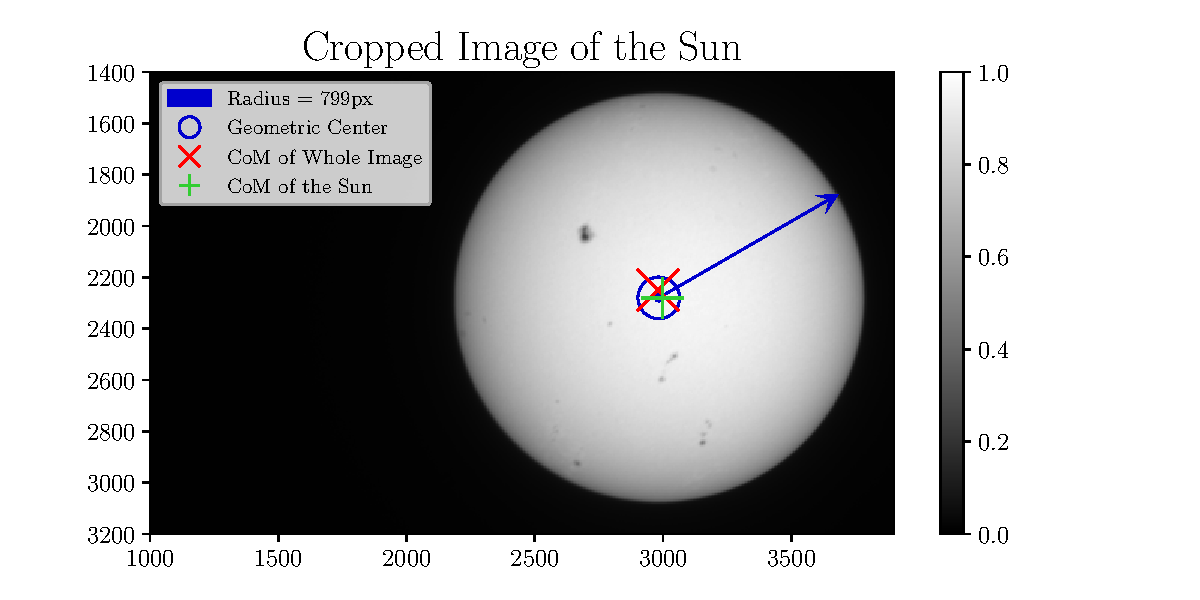
\includegraphics[width=\linewidth]{../fig/sun}
		\caption{تصویر بردیده‌شده خورشید با مشخص کردن شعاع و مرکزهای پیداشده با روش‌های مختلف.}
	\end{figure}
	
	\section{پروفایل روشنایی و تقریب ادینگتون}
	برای گرفتن پروفایل روشنایی، کافی است شعاع افقی به سمت راست (ساعت ۳) را در نظر بگیریم. این شعاع به نظر لکه‌ای ندارد
	و داده‌گیری روی آن راحت‌تر است چون زاویه‌ای ندارد، پس الگوریتم خط‌کشی نیاز ندارد. برای مقایسه پروفایل روشنایی آن با
	تقریب ادینگتون، باید پارامتر $\mu$ را برحسب فاصله از مرکز قرص بدست آوریم. با کمی هندسه ساده،
	\begin{equation}
		\mu = \cos{\theta} = \sqrt{1-\sin{\theta}} = \sqrt{1-\frac{x^2}{r^2}}
	\end{equation}
	که $x$ فاصله در صفحه از مرکز قرص و $r$ شعاع خورشید است.
	
	با رسم پروفایل روشنایی برحسب $\mu$ و مقایسه آن با تقریب ادینگتون، می‌بینیم در $\mu$های کوچک این تقریب خوب نیست اما
	در $\mu$های بزرگ‌تر این تقریب به‌نسبت خوب است. با تنظیم شعاع خورشید برای بهینه کردن تقریب ادینگتون، می‌توانیم فیت‌شدن
	آن را بهتر کنیم که نشان می‌دهد مشکل خوب نبودن تقریب برای $\mu$های کوچک ربطی به خود تقریب ادینگتون ندارد و به دلیل
	مبهم بودن فرایند انتخاب لبه خورشید است.
	\begin{figure}
		\centering
		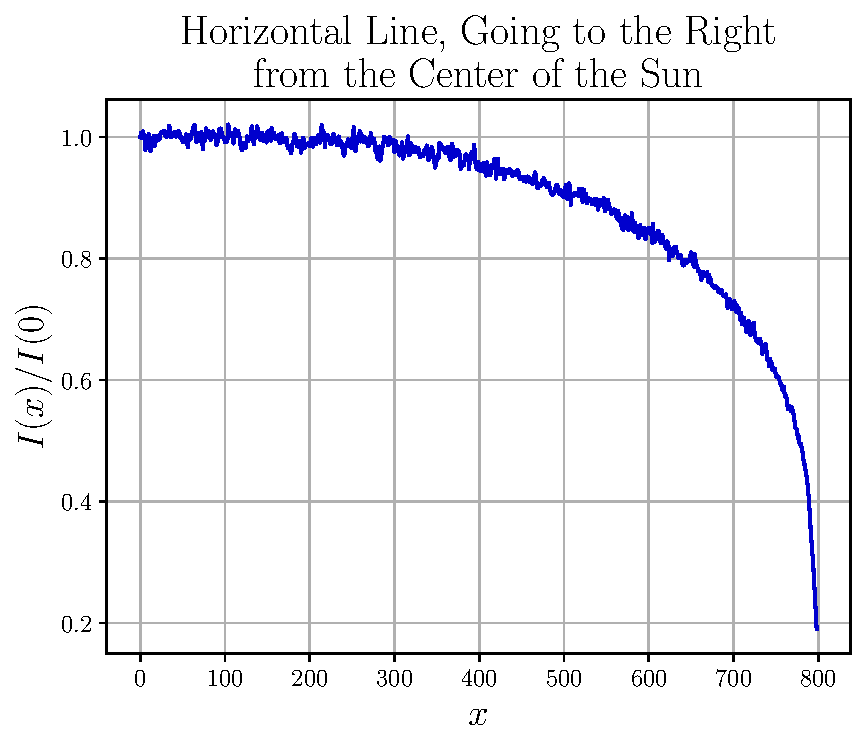
\includegraphics[width=0.8\linewidth]{../fig/intensity}
		\caption{پروفایل روشنایی برحسب فاصله از مرکز قرص}
	\end{figure}
	\begin{figure}
		\centering
		\begin{subfigure}{0.49\linewidth}
			\centering
			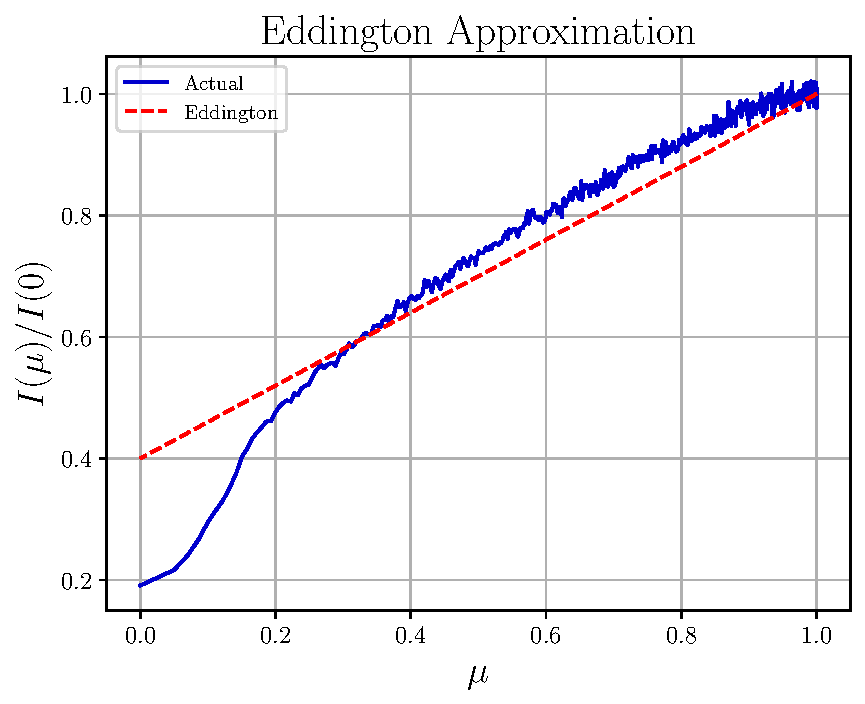
\includegraphics[width=\linewidth]{../fig/eddington}
		\end{subfigure}
		\begin{subfigure}{0.49\linewidth}
			\centering
			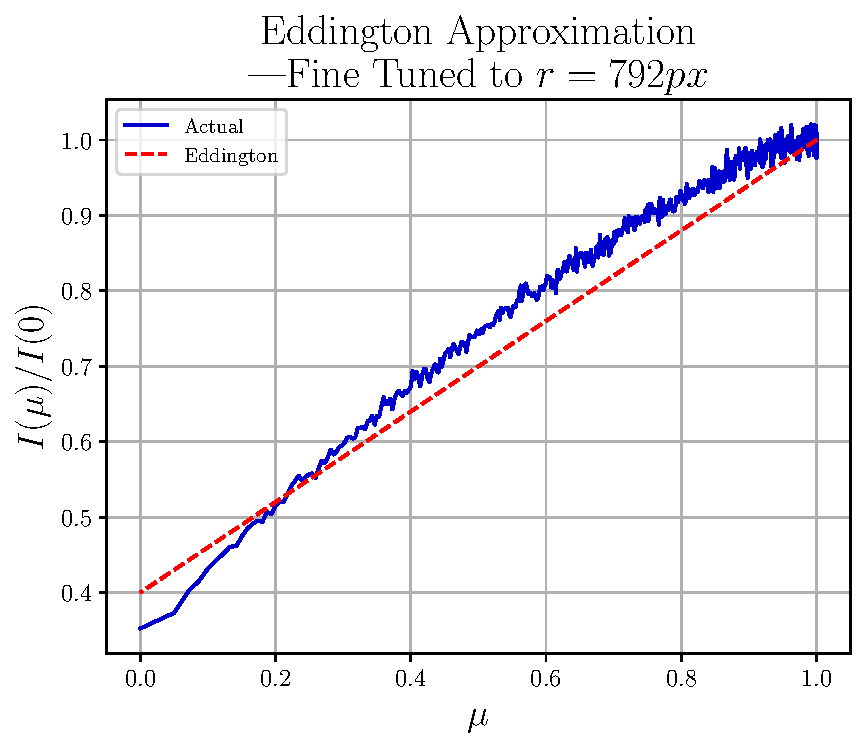
\includegraphics[width=\linewidth]{../fig/eddington-modified}
		\end{subfigure}
		\caption{مقایسه تقریب ادینگتون با دو شعاع متفاوت: شعاع بدست‌آمده از روشنایی و شعاع تنظیم‌شده.}
	\end{figure}
	
	\section{نمونه‌برداری روشنایی تصویر}
	در ناحیه کوچکی در وسط خورشید، میانگین و انحراف معیار روشنایی به ترتیب $10403$ و $101$ واحد (به ترتیب $95$ و $0.9$
	درصد در حالت بهنجار) هستند. در ناحیه کوچکی در گوشه‌های تصویر، دور از خورشید، میانگین و انحراف معیار روشنایی به
	ترتیب $43$ و $8$ واحد (به ترتیب $0.4$ و $0.07$ درصد در حالت بهنجار) هستند. مقادیر روشنایی دور از خورشید همچنان از
	نویز رندوم بزرگ‌تر هستند، چراکه روشنایی خورشید آنقدر زیاد است که این ناحیه را نیز تحت تأثیر قرار می‌دهد. همچنین
	با توجه به اعداد بدست آمده، واضح است که نسبت سیگنال به نویز داخل خورشید بیشتر از بیرون آن است که مطابق انتظارمان است.
	
	\section{نتیجه‌گیری}
	\begin{enumerate}
		\item تقریب ادینگتون به نسبت سادگی خود، دقت خوبی دارد، اما برای فیت کردن دقیق‌تر پروفایل روشنایی خورشید، باید ثوابت بهتری
		پیدا کنیم (به نظر می‌رسد پارامتر $\mu$ پارامتر خطی‌سازی مناسبی باشد).
		\item پیدا کردن لبه خورشید دقیق یا سرراست نیست و وابسته به کاربرد مورد نظرمان متفاوت است.
		\item روش هندسی برای پیداکردن مرکز خورشید از روش مرکز جرم دقیق‌تر است.
		\item نور خورشید، حتی از پشت فیلتر، بسیار شدید است و کل تصویر را تحت تأثیر قرار می‌دهد.
	\end{enumerate}
	 
\end{document}